\documentclass[11pt,a4paper]{article}
\usepackage[utf8]{inputenc}
\usepackage[top=0.70in, bottom=0.70in, left=0.8in,right=0.80in]{geometry}
\usepackage[pdftex]{graphicx}
\usepackage[bookmarks,colorlinks=false]{hyperref}
\hypersetup{pdfborder = {0 0 0}}
\usepackage[final]{pdfpages}
\usepackage{float}
\usepackage{array}
\usepackage{setspace}
\usepackage{enumerate}
\usepackage{longtable}
\usepackage[english]{babel}
\usepackage{amsmath}
\usepackage{pgfpages}
\usepackage{tikz}
\usetikzlibrary{arrows.meta,positioning,shapes.geometric,fit}
\usepackage{ragged2e}
\usepackage{titlesec}
\usepackage[font=large,labelfont=bf]{caption}
\def\figurename{\textbf{Figure }}
\usepackage[nottoc]{tocbibind}
\usepackage{acronym}
\usepackage{listings}
\usepackage{color}

\definecolor{dkgreen}{rgb}{0,0.6,0}
\definecolor{gray}{rgb}{0.5,0.5,0.5}
\definecolor{mauve}{rgb}{0.58,0,0.82}

\usepackage{fancyhdr}
\pagestyle{fancy}
\rhead{\large{AI Resume Builder}}
\fancyhead[L]{}
\fancyfoot[R]{\emph{Department of MCA}}
\fancyfoot[C]{\thepage}
\renewcommand{\headrulewidth}{0.5pt}
\renewcommand{\footrulewidth}{0.5pt}

\addto\captionsenglish{\renewcommand*\contentsname{\centering{Contents}}}
\addto\captionsenglish{
\renewcommand{\listfigurename}{\textit{List of Figures}}
}
\addto\captionsenglish{
\renewcommand{\listtablename}{\textit{List of Tables}}
}

\titleformat{\section}
  {\normalfont\Large\bfseries\raggedright}
  {\thesection}{1em}{}
\titleformat{\subsection}
  {\normalfont\large\bfseries\raggedright}
  {\thesubsection}{1em}{}
\titleformat{\subsubsection}
  {\normalfont\normalsize\bfseries\raggedright}
  {\thesubsubsection}{1em}{}

\newcommand{\resetbodyalignment}{
\par
\justifying
\leftskip=0pt
\rightskip=0pt
\parfillskip=0pt plus 1fil
\parindent=15pt
\normalfont\normalsize\selectfont
}

\begin{document}
\pagenumbering{roman}

\newpage
\begin{center}
\thispagestyle{empty}
\Large{\textbf{A MAJOR PROJECT REPORT \\ON}}\\[0.2cm]
\Large{\textsc{\textbf{``AI RESUME BUILDER''}}}\\
\vspace{0.1cm}

\includegraphics[scale=.5]{uop-logo}\\
\Large{\textbf{\\Submitted to}}
\LARGE{\textbf{\\ SAVITRIBAI PHULE PUNE UNIVERSITY\\}}
\large{\textbf{\\In Partial Fulfilment of the Requirement for the Award of\\}}
\Large{\textbf{\\ MASTER OF COMPUTER APPLICATIONS (Under Engineering)}}
\vspace{0.3cm}
\Large{\textbf{\\BY}}\\[0.1cm]
\begin{table}[h]
\centering
\Large{\textbf{
[Student Name]\\
Exam Seat No: [Seat Number]
}}
\end{table}
\large{\textbf{UNDER THE GUIDANCE OF}}\\
\Large{\textbf{[Guide Name]}}\\[0.1cm]

\includegraphics[scale=0.3]{tae.png}\\[.5cm]
\large{\textbf{DEPARTMENT OF MASTER OF COMPUTER APPLICATIONS}}\\
\Large{\textbf{TRINITY ACADEMY OF ENGINEERING}}\\[.5cm]
\large{\textbf{Kondhwa Annex, Pune - 411048}}
\large{\textbf{\\2024-2025}}\\
\newpage
\end{center}

\newpage

\begin{center}
\thispagestyle{empty}
\LARGE{\textbf{TRINITY ACADEMY OF ENGINEERING}} \\
\large{\textbf{Department of Master of Computer Applications}}\\

\includegraphics[scale=0.3]{tae.png}\\[1cm]
{\Huge \textbf{CERTIFICATE}}\\[0.5cm]
\end{center}
\linespread{1.13}
\begin{center}
\large{This is to certify that the Major Project entitled}\\[0.2cm]
\textbf{\Large{`AI RESUME BUILDER'}}\\
{has been successfully submitted by}\\
\begin{table}[h]
\centering
\large{\textbf{
[Student Name]\\
Exam Seat No: [Seat Number]
}}
\end{table}
under the supervision of \textbf{[Guide Name]} and it is approved for the partial fulfillment of the
requirement of Savitribai Phule Pune University, for the award of the degree of Master of
Computer Applications (Under Engineering).\\[0.5cm]
\end{center}
\large{\textbf{Date:\hspace*{0.4cm}/\hspace*{0.4cm}/}}\\[.2cm]
\large{\textbf{Place: Pune}}\\
\begin{spacing}{0}
\vspace*{1.2cm}
\hspace*{0.3in}\large{\textbf{[Guide Name]}}\hspace {1.1in}\large{\textbf{Dr. A. A. Bhusari}}\hspace*{1 in}\large{\textbf{Dr. R. J. Patil}}\\[.1cm]
\hspace*{0.4in}\textbf{Project Guide}\hspace*{1.8in}\textbf{HOD} \hspace*{1.5in}\textbf{Principal}\\
\hspace*{0.1 in}\textbf{Department of MCA}\hspace*{.8in}\textbf{Department of MCA} \hspace*{.9in}\textbf{TAE, Pune}\\[1 cm]
This project report has been examined by us as per the Savitribai Phule Pune University, Pune,
requirements at Trinity Academy of Engineering, Pune.
\\[2 cm]
\hspace*{0.5in}\textbf{Internal Examiner} \hspace*{2.6in}\textbf{External Examiner}\\[1cm]
\end{spacing}

\addcontentsline{toc}{section}{\textit{Certificate}}
\newpage

\begin{center}
\thispagestyle{plain}
\LARGE{\textbf{Acknowledgement}}\\[1cm]
\end{center}
\linespread{1.13}
\large{
\noindent
I would like to acknowledge all the teacher and friends who ever helped and assisted me throughout my project work.\newline \newline
First of all I would like to thank my respected guide \textbf {Guide Name}, introducing me throughout features needed. The time-to-time guidance, encouragement and valuable suggestion received from him are unforgettable in my life. This work would not have been possible without the enthusiastic response, insight and new idea from him.\newline \newline
Furthermore, I would like to thank respected \textbf{Dr. R. J. Patil}, Principal and  \textbf{Dr. A. A. Bhusari}, Head of Department of Master of Computer Applications for the guidance provided by them during my project work. I am also grateful to all the faculty members of Trinity Academy of Engineering, Pune for their support and cooperation. I would like to thank my lovely parent for time-to-time support and encouragement and valuable suggestion, and I would specify like to thank all my friends for their valuable suggestion and support. The acknowledgement world be incomplete without mention of the blessing of the almighty, which helped me in keeping high moral during difficult period.
}
\large{

\begin{flushright}
{
\textbf {\vspace{2.1cm}\\Student Name}
\textbf {\vspace{.1cm}\\Seat Number:4444}
\textbf {\vspace{.1cm}\\Department of MCA}
}
\end{flushright}
\par
}
%\newpage

\addcontentsline{toc}{section}{\textit{Acknowledgements}}
\newpage

\begin{center}
\thispagestyle{plain}
\vspace{1.8cm}
{\LARGE \textbf{\vspace{1.8cm}\\Declaration by the candidate}}\\[0.5cm]
\end{center}
\linespread{1.13}
\large{I hereby declare that this project report titled ``AI Resume Builder'' submitted towards partial fulfillment of requirements
for the degree of MCA is an authentic record of my work carried out under the guidance of \textbf{[Guide Name]}.
\\
I further declare that the material obtained from other resources is duly acknowledged in this report.
}\\[1.5cm]
\large{\textbf{Date:   \hspace*{0.1cm}/ \hspace*{0.1cm}/}}\\
\vspace*{0.8cm}
\large{\textbf{Place: Pune}\\
\begin{flushright}
{
\textbf{\vspace{2.2cm}\\[Student Name]}
\textbf{\vspace{.1cm}\\Seat Number: [Seat Number]}
\textbf{\vspace{.1cm}\\Department of MCA}
}
\end{flushright}
}

\addcontentsline{toc}{section}{\textit{Declaration}}
\newpage

\begin{center}
\thispagestyle{plain}
\vspace{2cm}
\LARGE{\textbf{Abstract}}\\[1.0cm]
\end{center}
Resume creation is a repetitive and error-prone activity for students, freshers, and working professionals, especially when they need multiple role-specific versions of the same profile. Many users struggle to translate free-form experience into a structured resume, understand how well their resume matches a job description, and prepare recruiter-ready supporting material such as cover emails or interview responses. This project addresses that gap by developing an AI Resume Builder that combines resume authoring, resume evaluation, job matching, interview preparation, and profile-based storage within a single web application.

The implemented system uses a React frontend and a Spring Boot backend connected through REST APIs. AI-assisted generation is performed through Spring AI with Ollama-hosted language models, while uploaded PDF and DOCX resumes are parsed and scored to produce ATS-style feedback. The platform supports user authentication, multiple resume templates, PDF export, saved resume history, live job search, and interview question generation. The result is a practical end-to-end tool that reduces manual formatting effort, improves resume quality, and gives users faster feedback during job preparation.

\newline \newline
\textit{{\textbf{Keywords: }} AI Resume Builder, resume generation, ATS analysis, Spring Boot, React, Ollama, PDF export.}

\addcontentsline{toc}{section}{\textit{Abstract}}
\newpage

\pagestyle{empty}
\tableofcontents
\newpage
\listoffigures
\newpage
\listoftables
\newpage

\thispagestyle{plain}
\section*{List of Abbreviation}
\begin{acronym}[SPRINGAI]
\acro{AIRB}{AI Resume Builder}
\acro{ATS}{Applicant Tracking System}
\acro{API}{Application Programming Interface}
\acro{UI}{User Interface}
\acro{JPA}{Java Persistence API}
\acro{LLM}{Large Language Model}
\acro{PDF}{Portable Document Format}
\acro{CORS}{Cross-Origin Resource Sharing}
\acro{REST}{Representational State Transfer}
\acro{SPRINGAI}{Spring AI}
\end{acronym}

\addcontentsline{toc}{section}{\textit{List of Abbreviation}}
\newpage
\cleardoublepage

\pagestyle{fancy}
\pagenumbering{arabic}

\resetbodyalignment
\section{About Project}
\subsection{Title}
\noindent The title of the project is \textbf{AI Resume Builder}.

\subsection{Domain}
\noindent The project belongs to the domains of artificial intelligence, full-stack web application development, and career support systems.

\subsection{Aim}
\begin{itemize}
\item To provide a single platform for generating structured resumes from unstructured user input.
\item To help users tailor resumes against job descriptions and identify missing keywords.
\item To support professional job preparation with interview questions, email drafting, and profile-based resume history.
\item To reduce manual effort in formatting, exporting, and maintaining multiple resume versions.
\item To combine AI-assisted writing with practical recruiter-facing workflows in one application.
\end{itemize}

\subsection{Objectives}
\begin{itemize}
\item Build a responsive frontend using React and Vite for resume creation, editing, and preview \cite{react_docs,vite_docs}.
\item Develop a Spring Boot backend that exposes secure endpoints for generation, upload analysis, profile access, and job search \cite{spring_boot_docs,spring_security_docs}.
\item Integrate Ollama through Spring AI to generate resumes, tailoring insights, and interview support \cite{spring_ai_docs,ollama_docs}.
\item Support upload-based ATS-style analysis for TXT, PDF, and DOCX resumes by using PDFBox, pdf.js, and Apache POI \cite{pdfbox_docs,pdfjs_docs,poi_docs}.
\item Enable template selection, PDF export, and saved resume history for authenticated users.
\end{itemize}

\subsection{Problem Statement}
\noindent Candidates often maintain resumes in static documents that are difficult to update, customize, or compare against job descriptions. Existing lightweight resume tools usually stop at formatting, while AI writing tools rarely provide structured templates, score-based review, saved history, and interview preparation in one consistent workflow. The problem addressed by this project is the lack of an integrated system that can generate a well-structured resume, adapt it for a target role, evaluate uploaded resumes, and preserve multiple recruiter-ready versions for future use.

\newpage
\resetbodyalignment
\section{Introduction}
\subsection{Overview}
\noindent AI Resume Builder is a web-based application designed to help users move from rough self-description to a complete, editable, and exportable resume. The frontend provides guided forms, prompt-based generation, template previews, and result screens, while the backend manages AI requests, file processing, user accounts, and persistence. The project is organized as a modern client-server system with React on the presentation layer and Spring Boot on the application layer \cite{react_docs,spring_boot_docs}.

\subsection{Motivation}
\noindent The job application process demands high-quality resumes that are concise, role-specific, and easy for both recruiters and automated screening systems to understand. Students and early-career candidates often do not know how to structure achievements, quantify impact, or identify missing keywords in a job description. This project was motivated by the need to make resume preparation faster, more accessible, and more adaptive by combining AI assistance with practical tools such as template switching, PDF export, uploaded resume scoring, and interview question generation.

\subsection{Project Scope \& Limitations}
\noindent The system covers resume generation, job-description matching, resume rating, interview question generation, email drafting, live job feed access, and user profile storage. The application supports multiple resume templates and can save role-specific versions for authenticated users. Its AI-assisted features depend on model availability and the quality of user-provided input. Live job listings also depend on external data providers. The project improves productivity and quality, but it does not replace domain-specific human review for final hiring decisions.

\subsection{Methodologies of Problem-Solving}
\noindent The solution follows a layered problem-solving methodology. First, user needs are translated into structured modules such as generation, scoring, storage, and search. Second, each module is implemented through a dedicated frontend workflow and backend endpoint. Third, AI prompts are constrained so that the model returns structured data that can be rendered consistently in templates. Fourth, file-based resume analysis is added to evaluate existing resumes instead of only generated ones. Finally, testing is used to validate navigation, API responses, error handling, and content persistence across the complete workflow.

\newpage
\resetbodyalignment
\section{Literature Survey}
\subsection{Similar Work}
\noindent Conventional resume builders generally focus on data entry and visual formatting, while AI writing tools focus on text generation without providing stable document structure, saved profile history, or ATS-style review. Job platforms offer listings, but they do not usually help users transform their experience into a tailored resume. Interview preparation tools are also commonly separated from resume authoring. The present project studies these disconnected workflows and combines them into one application so that the candidate can move from profile description to application-ready material without switching systems.

\noindent In recent software systems, three broad trends are visible. The first trend is document automation, where a system helps users create documents quickly through templates and reusable layouts. The second trend is AI-assisted writing, where a language model converts rough notes into professional text. The third trend is job-preparation intelligence, where resume scoring, keyword matching, and interview guidance are treated as separate supporting tools. The proposed AI Resume Builder is motivated by the observation that candidates usually need all three capabilities together, not as isolated products. Because of that, the project deliberately joins authoring, evaluation, and job-readiness into one consistent workflow.

\subsection{Review of Existing Approaches}
\noindent Traditional resume generators are useful when the user already knows how to describe projects, quantify achievements, and organize sections properly. Their strength lies in predictable layouts and export quality, but they do little to improve the actual content quality of the resume. In contrast, AI content tools can rephrase responsibilities and produce summaries, yet their raw output may be inconsistent, verbose, or not aligned with a recruiter-friendly structure.

\noindent ATS-style scanners introduced another layer of support by checking whether a resume contains measurable outcomes, action verbs, and role-relevant keywords. However, these scanners commonly operate only after a resume has already been written. Users are then forced to switch back to a separate builder or word processor to make the suggested changes. This back-and-forth workflow becomes inefficient when multiple job-specific versions are required.

\noindent Live job boards and interview preparation assistants have also become common in career-support platforms. Even so, job discovery, resume customization, and interview preparation remain disconnected steps. The candidate may discover a role on one platform, rewrite the resume on another, and prepare questions on a third. The literature survey therefore supports the need for a unified application where each step can reuse the same underlying profile data.

\subsection{Tabulated Short Survey}
\begin{table}[H]
\centering
\caption{Short survey of existing solution categories}
\begin{tabular}{|p{3.1cm}|p{4.2cm}|p{5.0cm}|}
\hline
\textbf{Category} & \textbf{Strengths} & \textbf{Observed Limitations} \\
\hline
Template-only resume builders & Fast layout generation and printable output & Limited personalization, no AI drafting, and weak job-specific adaptation \\
\hline
Generic AI writing tools & Good text expansion and rewriting support & Output is often unstructured and not directly ready for resume templates \\
\hline
Standalone ATS scanners & Helpful for keyword and section feedback & Usually require a separate resume creation workflow and manual correction \\
\hline
Job portals & Provide role discovery and application links & Do not convert candidate data into a strong resume or interview preparation plan \\
\hline
Interview prep tools & Useful for question practice and readiness & Commonly disconnected from actual resume content and target job context \\
\hline
\end{tabular}
\end{table}

\begin{table}[H]
\centering
\caption{Comparative view of major support capabilities}
\begin{tabular}{|p{3.4cm}|p{2.0cm}|p{2.0cm}|p{2.0cm}|p{2.0cm}|}
\hline
\textbf{System Type} & \textbf{AI Drafting} & \textbf{Template Output} & \textbf{ATS Review} & \textbf{Profile History} \\
\hline
Basic resume builders & Low & High & Low & Low \\
\hline
Generic AI tools & High & Low & Low & Low \\
\hline
ATS scanners & Low & Low & High & Low \\
\hline
Job portals & Low & Low & Medium & Low \\
\hline
AI Resume Builder & High & High & High & High \\
\hline
\end{tabular}
\end{table}

\subsection{Advantages and Disadvantages of Previous System}
\noindent Previous systems are strong in isolated tasks, such as layout design, keyword scanning, or job listing aggregation. However, they typically make the user move between multiple tools to finish one application cycle. This increases friction, duplicates effort, and makes it harder to maintain consistency across resume content, job targeting, and interview preparation. The main disadvantage of the older fragmented approach is the lack of one reliable source of truth for the candidate profile.

\noindent Another limitation of earlier systems is the absence of structured iteration. Users often receive feedback such as ``add stronger action verbs'' or ``improve keyword coverage,'' but the tool that produced the feedback is not the same tool that helps them rewrite the content. As a result, improvements are manual and error-prone. Moreover, many previous systems treat the final resume as a static file instead of a reusable data model. That makes it difficult to generate several variants of the same profile for different job roles.

\subsection{Research Gap}
\noindent The main gap identified from the survey is the lack of integration between content generation, structured editing, resume evaluation, and candidate support services. Many existing platforms specialize in only one part of the problem. Very few systems let a user begin with a free-form profile description, transform it into structured resume sections, evaluate it against a role, save alternate versions, and continue into interview preparation without re-entering the same data repeatedly.

\noindent A second gap concerns local and controllable AI usage. Some tools rely completely on remote hosted models, which may introduce cost, latency, or privacy concerns. By using Spring AI with Ollama, the proposed project explores a more developer-controlled deployment pattern while still preserving practical usefulness for students and job seekers.

\subsection{Outcome of Literature Survey}
\noindent The literature survey indicates that an effective resume platform should unify structured authoring, AI enhancement, evaluation, and storage. Therefore, the proposed system integrates resume generation, upload-based review, job-description matching, interview question generation, and saved resume profiles in one architecture. The technical stack selected for this integration is also well supported by mature frontend, backend, AI, and document-processing ecosystems \cite{spring_ai_docs,pdfbox_docs,poi_docs}.

\noindent The survey also justifies the architectural direction of this project. React is appropriate for fast interactive UI iteration, Spring Boot provides stable API and service orchestration, Spring AI simplifies model integration, and PDF/DOCX processing libraries make file-based review practical. Hence, both the product concept and the technical stack are supported by the needs observed in current resume-building workflows.

\newpage
\resetbodyalignment
\section{Software Requirements Specification}
\subsection{Functional Requirement}
\subsubsection{System Features}
\begin{itemize}
\item Generate a structured resume from a free-form candidate description and optional job description.
\item Allow manual editing of personal details, skills, experience, education, projects, and certifications.
\item Provide multiple resume templates and support PDF export.
\item Analyze an uploaded TXT, PDF, or DOCX resume and return ATS-style feedback.
\item Generate interview questions from resume content, target role, and job context.
\item Support sign up, sign in, profile access, and saved resume history.
\item Offer live job search and company profile assistance through backend-integrated external feeds.
\item Generate professional email drafts to support application outreach.
\end{itemize}

\subsubsection{Detailed Functional Modules}
\begin{table}[H]
\centering
\caption{Detailed functional modules of the system}
\begin{tabular}{|p{3.5cm}|p{8.6cm}|}
\hline
\textbf{Module} & \textbf{Expected Behavior} \\
\hline
User authentication & Register new users, validate login credentials, create session tokens, and restrict access to profile-only features. \\
\hline
Resume generation & Accept a candidate summary and optional job description, send prompt to AI layer, and return structured JSON for resume sections. \\
\hline
Resume editor & Let the user update generated content manually for projects, education, skills, links, and experience bullets. \\
\hline
Template and export & Render the same resume data in multiple templates and export the chosen version to PDF. \\
\hline
ATS-style rating & Read uploaded resume content and evaluate section completeness, impact language, and keyword presence. \\
\hline
Profile persistence & Save selected resume versions with file name, template selection, and styling configuration. \\
\hline
Interview preparation & Generate role-aware interview questions and preparation guidance using the same resume context. \\
\hline
Jobs support & Fetch live jobs and related company details to help users continue from resume creation into job search. \\
\hline
\end{tabular}
\end{table}

\subsubsection{Primary Use Cases}
\begin{itemize}
\item A user enters a free-form description and receives a first draft of the resume.
\item A user pastes a target job description and requests better role alignment.
\item A user uploads an existing resume to check its quality and missing keywords.
\item A signed-in user saves a generated resume version and reopens it later.
\item A user explores live job opportunities and prepares likely interview questions.
\end{itemize}

\subsection{External Interface Requirement}
\subsubsection{User Interface}
\begin{itemize}
\item Responsive web interface with dedicated pages for landing, resume generation, resume rating, interview preparation, job search, login, and profile management.
\item Form-based editing, AI prompt input, template selection, and download actions.
\item Clear validation and error feedback for upload failures, missing fields, and unavailable AI services.
\end{itemize}

\subsubsection{Software Interface}
\begin{itemize}
\item Frontend: React 19, Vite 6, Tailwind CSS, axios, react-router-dom, jsPDF, pdf.js \cite{react_docs,vite_docs,jspdf_docs,pdfjs_docs}.
\item Backend: Spring Boot 3.4.2, Spring Data JPA, Spring Security, Spring AI, Apache POI, Apache PDFBox \cite{spring_boot_docs,spring_data_docs,spring_security_docs,spring_ai_docs,poi_docs,pdfbox_docs}.
\item AI Layer: Ollama-hosted model served through Spring AI \cite{ollama_docs,spring_ai_docs}.
\item Database Layer: relational persistence for users and saved resumes, with deployable MySQL support and H2-based local development configuration.
\end{itemize}

\subsubsection{Communication Interfaces}
\begin{itemize}
\item REST APIs over HTTP between the React client and Spring Boot backend.
\item Header-based session token handling for authenticated profile endpoints.
\item External HTTP integration for live job feeds and optional external interview model access.
\end{itemize}

\subsection{Input and Output Specification}
\subsubsection{Input Specification}
\begin{itemize}
\item Candidate summary text describing education, skills, projects, and experience.
\item Optional job description used for tailoring and keyword alignment.
\item Resume files in TXT, PDF, or DOCX format for rating workflow.
\item Login and sign-up data such as name, email, and password.
\item User selections such as template choice, color accent, and target role.
\end{itemize}

\subsubsection{Output Specification}
\begin{itemize}
\item Structured resume JSON ready for editing and rendering.
\item Resume preview rendered in multiple template formats.
\item PDF export of the chosen resume layout.
\item ATS-style scoring output with strengths, improvements, and keyword guidance.
\item Saved profile records containing previously generated resume versions.
\item Interview question sets and live job result lists.
\end{itemize}

\subsection{Nonfunctional Requirements}
\subsubsection{Performance Requirements}
\noindent The system should return normal UI actions immediately and AI-assisted responses within an acceptable interactive wait time. Cached job search responses and structured prompt handling are used to keep the experience consistent.

\subsubsection{Safety Requirements}
\noindent The application should validate file uploads, reject unsupported formats, and handle unavailable upstream services without crashing the user workflow.

\subsubsection{Security Requirements}
\noindent User accounts require authenticated access for profile storage. Passwords are stored as hashes, session tokens are validated on protected routes, and CORS is explicitly configured for approved frontend origins \cite{spring_security_docs}.

\subsubsection{Software Quality Attributes}
\noindent The solution emphasizes usability, modularity, maintainability, and extensibility. Separate controllers, services, repositories, and frontend page modules make it easier to add future features without rewriting the entire system.

\subsubsection{Reliability and Availability}
\noindent The application should remain usable even when an external dependency is unavailable. For example, manual resume editing should still work when the AI service is down, and informative error messages should be shown instead of blank screens. This requirement is important because the project depends on both model availability and external job feeds.

\subsubsection{Scalability Considerations}
\noindent The current academic project is targeted at moderate single-user or small-group usage. However, the layered architecture supports future scaling by separating frontend rendering, business services, AI orchestration, and data persistence. Caching, externalized configuration, and independent service modules make future optimization possible.

\subsection{System Requirement}
\subsubsection{Database Requirement}
\begin{itemize}
\item Relational database support for user accounts and saved resumes.
\item MySQL for deployment-oriented persistence and H2 for local/test configuration.
\end{itemize}

\subsubsection{Software Requirement}
\begin{itemize}
\item Windows 11 or equivalent development environment.
\item Java 21 and Maven for backend execution.
\item Node.js and npm for frontend execution.
\item Web browser such as Chrome or Edge.
\item Ollama runtime for local LLM execution.
\end{itemize}

\subsubsection{Hardware Requirement}
\begin{itemize}
\item Laptop or desktop computer.
\item Minimum 4 GB RAM, with higher memory preferred for local AI model usage.
\item Stable internet connectivity for live job feeds and package installation.
\end{itemize}

\subsection{Assumptions and Constraints}
\subsubsection{Assumptions}
\begin{itemize}
\item The user provides meaningful profile information for high-quality AI output.
\item Ollama or the configured model endpoint is available during AI-assisted operations.
\item The browser supports modern JavaScript required by the React-based frontend.
\item Uploaded resumes contain extractable text rather than only scanned image content.
\end{itemize}

\subsubsection{Constraints}
\begin{itemize}
\item AI output quality depends on prompt quality and the chosen underlying model.
\item External jobs data depends on the availability and policy of upstream providers.
\item Local machine performance can affect the response time of AI generation and PDF processing.
\item The current version focuses on English-language resume content and recruiter-style formatting.
\end{itemize}

\subsection{Analysis Model}
\subsubsection{SDLC Model to be Applied}
\begin{figure}[H]
\centering
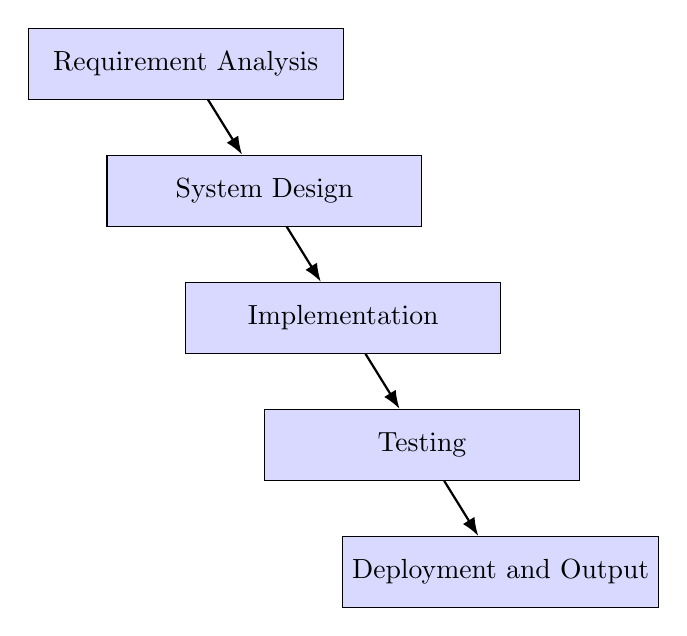
\begin{tikzpicture}[
  stage/.style={draw, fill=blue!15, minimum width=4cm, minimum height=0.9cm, align=center},
  arrow/.style={-Latex, thick}
]
\node[stage] (a) {Requirement Analysis};
\node[stage, below=0.7cm of a, xshift=1.0cm] (b) {System Design};
\node[stage, below=0.7cm of b, xshift=1.0cm] (c) {Implementation};
\node[stage, below=0.7cm of c, xshift=1.0cm] (d) {Testing};
\node[stage, below=0.7cm of d, xshift=1.0cm] (e) {Deployment and Output};
\draw[arrow] (a) -- (b);
\draw[arrow] (b) -- (c);
\draw[arrow] (c) -- (d);
\draw[arrow] (d) -- (e);
\end{tikzpicture}
\caption{Applied SDLC model for the AI Resume Builder project}
\end{figure}

\subsubsection{Requirement Traceability Overview}
\begin{table}[H]
\centering
\caption{Traceability from need to implemented module}
\begin{tabular}{|p{4.2cm}|p{4.6cm}|p{3.4cm}|}
\hline
\textbf{User Need} & \textbf{Implemented Module} & \textbf{Verification} \\
\hline
Need resume quickly from rough notes & Resume generation endpoint and form UI & Functional testing \\
\hline
Need better alignment with job role & Job-match and tailoring workflow & API and UI testing \\
\hline
Need to improve existing resume & Upload and ATS rating module & File handling tests \\
\hline
Need multiple saved versions & Profile and saved resume persistence & Authentication and save tests \\
\hline
Need application support beyond resume & Email, jobs, and interview modules & End-to-end flow review \\
\hline
\end{tabular}
\end{table}

\newpage
\resetbodyalignment
\section{Project Plan}
\subsection{Project Estimate}
\subsubsection{Reconciled Estimates}
\begin{table}[H]
\centering
\caption{High-level project schedule}
\begin{tabular}{|p{5.0cm}|p{3.2cm}|p{3.2cm}|}
\hline
\textbf{Activity} & \textbf{Planned Duration} & \textbf{Outcome} \\
\hline
Requirement analysis and feature selection & 1 week & Finalized module list and stack choice \\
\hline
Frontend structure and routing & 2 weeks & Core pages and navigation flow \\
\hline
Backend API and database modules & 2 weeks & Auth, resume, profile, and jobs endpoints \\
\hline
AI workflow integration & 1 week & Resume, email, and interview generation \\
\hline
Testing and refinement & 1 week & Error handling, validation, and content review \\
\hline
Documentation and report preparation & 1 week & Final report and project packaging \\
\hline
\end{tabular}
\end{table}

\subsubsection{Project Resources}
\begin{itemize}
\item Development resources: Java 21, Maven, Node.js, npm, Vite, Spring Boot, and Git.
\item AI resources: Ollama runtime and prompt templates for resume and interview tasks.
\item Persistence resources: JPA repositories, relational database storage, and JSON serialization for saved resumes.
\item Documentation resources: official framework documentation, internal README, and test outputs.
\end{itemize}

\subsection{Risk Management}
\subsubsection{Risk Identification}
\begin{itemize}
\item AI model unavailability or slow local inference.
\item Invalid uploaded files or unreadable resume content.
\item Authentication or profile persistence failures.
\item External live job data source changes or downtime.
\item Output inconsistency when user input is too short or ambiguous.
\end{itemize}

\subsubsection{Risk Analysis}
\noindent The highest risks are concentrated around AI dependency, external API dependency, and data quality. These do not usually affect static page rendering, but they directly affect the smart features that define the product value.

\subsubsection{Overview of Risk Mitigation, Monitoring, Management}
\begin{table}[H]
\centering
\caption{Risk mitigation summary}
\begin{tabular}{|p{4.0cm}|p{3.4cm}|p{5.0cm}|}
\hline
\textbf{Risk} & \textbf{Impact} & \textbf{Mitigation} \\
\hline
Ollama service unavailable & High & Show service error, keep manual editing workflow available \\
\hline
Malformed upload files & Medium & Validate file types and provide readable upload error messages \\
\hline
Weak user prompts & Medium & Enforce minimum input and allow manual corrections after generation \\
\hline
External job API changes & Medium & Keep fallback source and isolate live job logic in service layer \\
\hline
Session/token expiry & Low to medium & Guard profile endpoints and redirect users to sign in again \\
\hline
\end{tabular}
\end{table}

\newpage
\resetbodyalignment
\section{System Design}
\subsection{System Architecture}
\noindent The project follows a client-server architecture. The React frontend handles routing, forms, previews, and template interaction. The Spring Boot backend provides REST endpoints for resume generation, job matching, profile storage, authentication, upload analysis, and job search. AI-assisted features are routed through Spring AI to Ollama, while persistence is handled through JPA repositories and relational tables for users and saved resumes.

\begin{figure}[H]
\centering
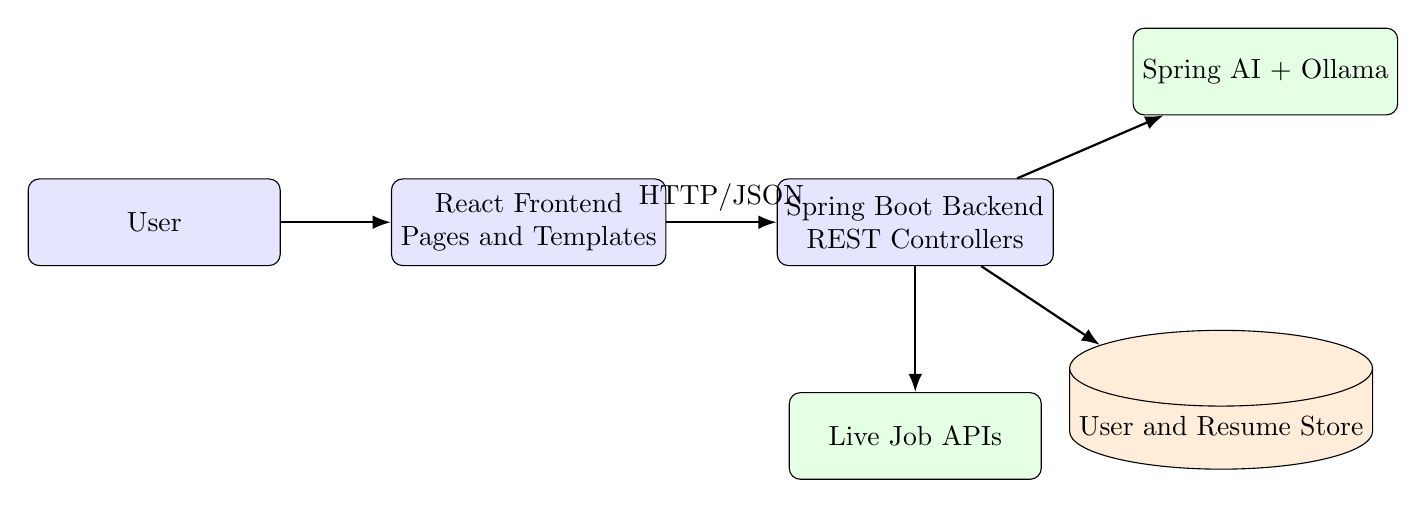
\begin{tikzpicture}[
  box/.style={draw, rounded corners, minimum width=3.2cm, minimum height=1.1cm, align=center, fill=blue!10},
  ext/.style={draw, rounded corners, minimum width=3.2cm, minimum height=1.1cm, align=center, fill=green!10},
  data/.style={draw, cylinder, shape border rotate=90, aspect=0.25, minimum height=1.2cm, minimum width=2.4cm, align=center, fill=orange!15},
  arrow/.style={-Latex, thick}
]
\node[box] (user) {User};
\node[box, right=1.4cm of user] (frontend) {React Frontend\\Pages and Templates};
\node[box, right=1.4cm of frontend] (backend) {Spring Boot Backend\\REST Controllers};
\node[ext, above right=0.8cm and 1.0cm of backend] (ai) {Spring AI + Ollama};
\node[data, below right=0.9cm and 1.0cm of backend] (db) {User and Resume Store};
\node[ext, below=1.6cm of backend] (jobs) {Live Job APIs};
\draw[arrow] (user) -- (frontend);
\draw[arrow] (frontend) -- node[above]{HTTP/JSON} (backend);
\draw[arrow] (backend) -- (ai);
\draw[arrow] (backend) -- (db);
\draw[arrow] (backend) -- (jobs);
\end{tikzpicture}
\caption{High-level system architecture of AI Resume Builder}
\end{figure}

\subsection{Data Flow Diagrams}
\noindent The most important data flow starts with candidate input. The frontend sends the free-form description and optional job description to the backend. The backend prepares prompts, sends them to Ollama, converts the model response into structured JSON, and returns that payload to the frontend for editing, template rendering, and export.

\begin{figure}[H]
\centering
\begin{tikzpicture}[
  step/.style={draw, minimum width=3.2cm, minimum height=0.9cm, align=center, fill=cyan!12},
  arrow/.style={-Latex, thick}
]
\node[step] (a) {Enter candidate description};
\node[step, below=0.6cm of a] (b) {Submit to /api/v1/resume/generate};
\node[step, below=0.6cm of b] (c) {Prompt processing in backend};
\node[step, below=0.6cm of c] (d) {Ollama generates structured resume data};
\node[step, below=0.6cm of d] (e) {Frontend previews and edits result};
\node[step, below=0.6cm of e] (f) {Template selection and PDF export};
\draw[arrow] (a) -- (b);
\draw[arrow] (b) -- (c);
\draw[arrow] (c) -- (d);
\draw[arrow] (d) -- (e);
\draw[arrow] (e) -- (f);
\end{tikzpicture}
\caption{Resume generation data flow}
\end{figure}

\begin{figure}[H]
\centering
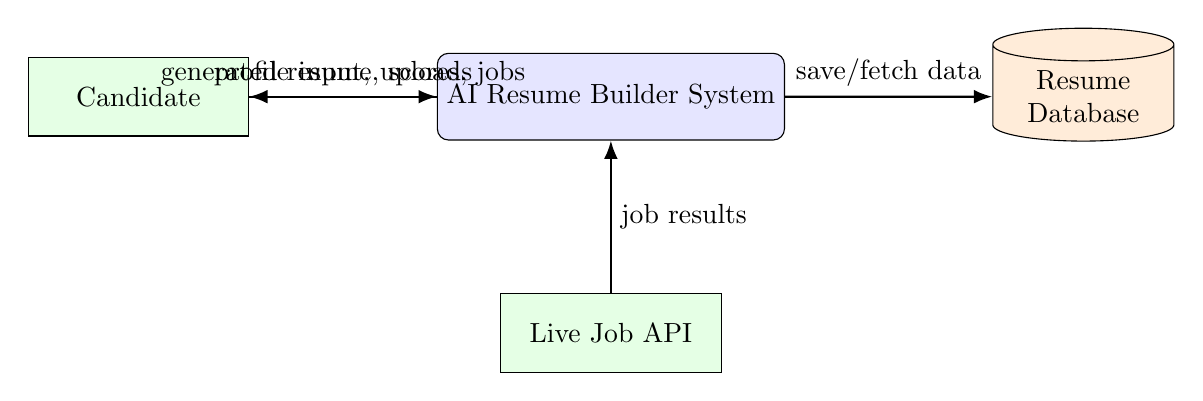
\begin{tikzpicture}[
  ext/.style={draw, minimum width=2.8cm, minimum height=1cm, align=center, fill=green!10},
  proc/.style={draw, rounded corners, minimum width=4.0cm, minimum height=1.1cm, align=center, fill=blue!10},
  store/.style={draw, cylinder, shape border rotate=90, aspect=0.25, minimum width=2.3cm, minimum height=1.2cm, align=center, fill=orange!15},
  arrow/.style={-Latex, thick}
]
\node[ext] (user) at (0,0) {Candidate};
\node[proc] (system) at (6,0) {AI Resume Builder System};
\node[store] (db) at (12,0) {Resume\\Database};
\node[ext] (jobs) at (6,-3) {Live Job API};
\draw[arrow] (user) -- node[above]{profile input, uploads} (system);
\draw[arrow] (system) -- node[above]{generated resume, scores, jobs} (user);
\draw[arrow] (system) -- node[above]{save/fetch data} (db);
\draw[arrow] (jobs) -- node[right]{job results} (system);
\end{tikzpicture}
\caption{DFD Level 1 for AI Resume Builder}
\end{figure}

\begin{figure}[H]
\centering
\begin{tikzpicture}[
  step/.style={draw, minimum width=3.4cm, minimum height=0.9cm, align=center, fill=purple!10},
  arrow/.style={-Latex, thick}
]
\node[step] (a) {User signs in};
\node[step, below=0.6cm of a] (b) {Session token sent in X-Auth-Token};
\node[step, below=0.6cm of b] (c) {Resume JSON and template posted};
\node[step, below=0.6cm of c] (d) {Backend stores saved resume record};
\node[step, below=0.6cm of d] (e) {Profile page loads saved history};
\draw[arrow] (a) -- (b);
\draw[arrow] (b) -- (c);
\draw[arrow] (c) -- (d);
\draw[arrow] (d) -- (e);
\end{tikzpicture}
\caption{Saved profile and resume history flow}
\end{figure}

\begin{figure}[H]
\centering
\begin{tikzpicture}[
  step/.style={draw, minimum width=3.8cm, minimum height=0.9cm, align=center, fill=yellow!15},
  arrow/.style={-Latex, thick}
]
\node[step] (a) {Upload resume file};
\node[step, below=0.6cm of a] (b) {Read TXT, PDF, or DOCX};
\node[step, below=0.6cm of b] (c) {Extract plain text content};
\node[step, below=0.6cm of c] (d) {Analyze ATS signals and keywords};
\node[step, below=0.6cm of d] (e) {Return score, strengths, and suggestions};
\draw[arrow] (a) -- (b);
\draw[arrow] (b) -- (c);
\draw[arrow] (c) -- (d);
\draw[arrow] (d) -- (e);
\end{tikzpicture}
\caption{Resume upload and ATS analysis flow}
\end{figure}

\begin{figure}[H]
\centering
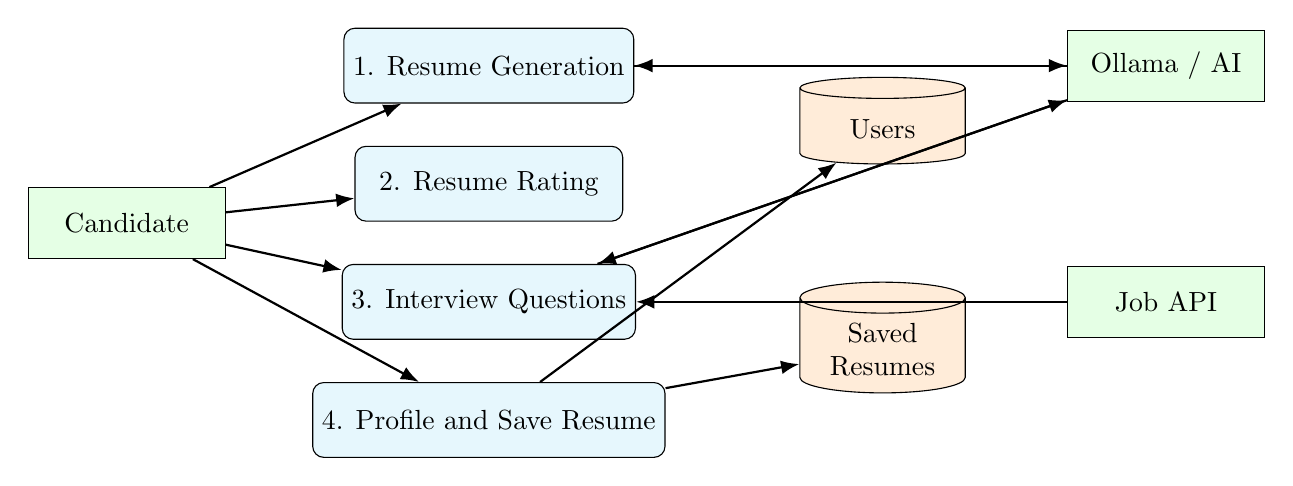
\begin{tikzpicture}[
  proc/.style={draw, rounded corners, minimum width=3.4cm, minimum height=0.95cm, align=center, fill=cyan!10},
  store/.style={draw, cylinder, shape border rotate=90, aspect=0.25, minimum width=2.1cm, minimum height=1.1cm, align=center, fill=orange!15},
  ext/.style={draw, minimum width=2.5cm, minimum height=0.9cm, align=center, fill=green!10},
  arrow/.style={-Latex, thick}
]
\node[ext] (user) at (0,0) {Candidate};
\node[proc] (p1) at (4.6,2.0) {1. Resume Generation};
\node[proc] (p2) at (4.6,0.5) {2. Resume Rating};
\node[proc] (p3) at (4.6,-1.0) {3. Interview Questions};
\node[proc] (p4) at (4.6,-2.5) {4. Profile and Save Resume};
\node[store] (d1) at (9.6,1.2) {Users};
\node[store] (d2) at (9.6,-1.6) {Saved\\Resumes};
\node[ext] (ai) at (13.2,2.0) {Ollama / AI};
\node[ext] (jobs) at (13.2,-1.0) {Job API};
\draw[arrow] (user) -- (p1);
\draw[arrow] (user) -- (p2);
\draw[arrow] (user) -- (p3);
\draw[arrow] (user) -- (p4);
\draw[arrow] (p1) -- (ai);
\draw[arrow] (ai) -- (p1);
\draw[arrow] (p3) -- (ai);
\draw[arrow] (ai) -- (p3);
\draw[arrow] (p4) -- (d1);
\draw[arrow] (p4) -- (d2);
\draw[arrow] (jobs) -- (p3);
\end{tikzpicture}
\caption{DFD Level 2 for AI Resume Builder}
\end{figure}

\subsection{Entity Relationship Diagram}
\noindent The persistence layer mainly stores user accounts and the resume versions saved by each user. Each user can save multiple generated resumes, while each saved resume belongs to exactly one user. The ER diagram below represents that relationship.

\begin{figure}[H]
\centering
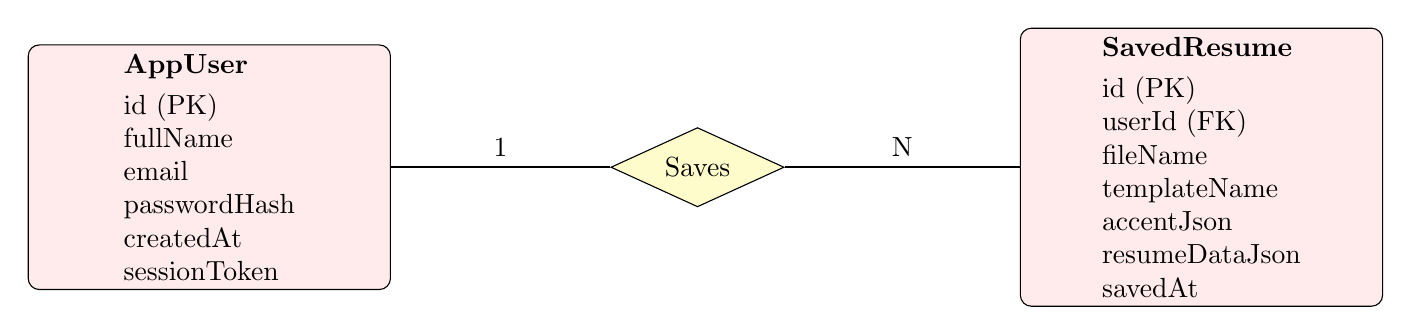
\begin{tikzpicture}[
  entity/.style={draw, rounded corners, minimum width=4.6cm, minimum height=2.2cm, align=left, fill=red!8},
  relation/.style={draw, diamond, aspect=2, minimum width=2.2cm, minimum height=1cm, align=center, fill=yellow!20},
  line/.style={thick}
]
\node[entity] (u) at (0,0) {\textbf{AppUser}\\[0.1cm]
id (PK)\\
fullName\\
email\\
passwordHash\\
createdAt\\
sessionToken};
\node[relation] (rel) at (6.2,0) {Saves};
\node[entity] (r) at (12.6,0) {\textbf{SavedResume}\\[0.1cm]
id (PK)\\
userId (FK)\\
fileName\\
templateName\\
accentJson\\
resumeDataJson\\
savedAt};
\draw[line] (u) -- node[above]{1} (rel);
\draw[line] (rel) -- node[above]{N} (r);
\end{tikzpicture}
\caption{ER diagram of user and saved resume entities}
\end{figure}

\subsection{UML Diagrams}
\noindent From a use-case perspective, the primary actor is the candidate. The candidate can create an account, generate a resume, upload an existing resume for analysis, choose a template, export the final PDF, save role-specific versions, browse job listings, and prepare for interviews. The backend supports these actions through dedicated controllers such as AuthController, ResumeController, ProfileController, JobSearchController, and InterviewQuestionController.

\begin{table}[H]
\centering
\caption{Primary use cases}
\begin{tabular}{|p{3.3cm}|p{8.8cm}|}
\hline
\textbf{Actor} & \textbf{Use Cases} \\
\hline
Candidate & Sign up, sign in, generate resume, edit sections, upload resume, rate resume, export PDF, save resume, browse jobs, generate interview questions, create professional email \\
\hline
System & Validate input, call AI services, parse files, persist saved resumes, return live job data, guard protected routes \\
\hline
\end{tabular}
\end{table}

\begin{figure}[H]
\centering
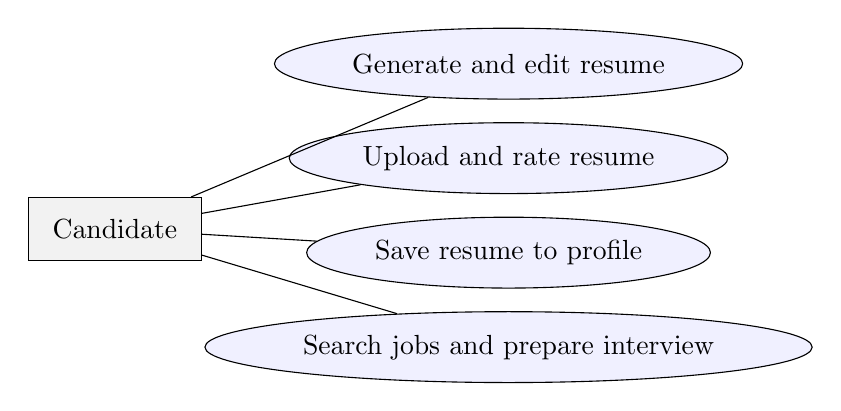
\begin{tikzpicture}[
  actor/.style={draw, minimum width=2.2cm, minimum height=0.8cm, align=center, fill=gray!10},
  usecase/.style={draw, ellipse, minimum width=4.2cm, minimum height=0.9cm, align=center, fill=blue!6}
]
\node[actor] (user) at (0,0) {Candidate};
\node[usecase] (gen) at (5,2.1) {Generate and edit resume};
\node[usecase] (rate) at (5,0.9) {Upload and rate resume};
\node[usecase] (save) at (5,-0.3) {Save resume to profile};
\node[usecase] (jobs) at (5,-1.5) {Search jobs and prepare interview};
\draw (user) -- (gen);
\draw (user) -- (rate);
\draw (user) -- (save);
\draw (user) -- (jobs);
\end{tikzpicture}
\caption{Simplified use-case diagram for the main user}
\end{figure}

\newpage
\resetbodyalignment
\section{Project Implementation}
\subsection{Implementation Overview}
\noindent The implementation is divided into frontend, backend, AI, and persistence modules. The frontend contains dedicated pages such as Home, Services, Generate Resume, Rate Resume, Interview Questions, Live Jobs Board, Login, and Profile. The backend exposes grouped REST endpoints for authentication, resume generation, upload analysis, email generation, interview question generation, profile operations, and live jobs search. This separation keeps presentation logic, domain logic, and persistence responsibilities independent.

\begin{table}[H]
\centering
\caption{Implementation modules}
\begin{tabular}{|p{3.3cm}|p{4.0cm}|p{4.8cm}|}
\hline
\textbf{Layer} & \textbf{Representative Modules} & \textbf{Responsibility} \\
\hline
Frontend & GenerateResume, RateResume, Profile, LiveJobsBoard & Data entry, preview, export, navigation, and interactive UI \\
\hline
Backend Controllers & AuthController, ResumeController, ProfileController & API entry points and request validation \\
\hline
Backend Services & ResumeService, UserAccountService, JobSearchService & AI orchestration, persistence logic, and upstream integrations \\
\hline
Persistence & AppUser, SavedResume, JPA repositories & Store users, session tokens, and saved resume payloads \\
\hline
AI and Parsing & Spring AI, Ollama, PDFBox, Apache POI, pdf.js & Generation, rating, PDF parsing, DOCX parsing, and structured extraction \\
\hline
\end{tabular}
\end{table}

\subsection{Resume Generation Workflow}
\noindent The central workflow begins with a free-form description of the candidate and an optional target job description. The backend uses Spring AI to send a structured prompt to Ollama, receives the response, and transforms it into JSON that matches resume sections such as personal information, summary, skills, experience, education, projects, and achievements. The frontend then renders the result in editable form and template previews \cite{spring_ai_docs,ollama_docs}.

\begin{figure}[H]
\centering
\begin{tikzpicture}[
  node distance=0.6cm,
  step/.style={draw, rounded corners, minimum width=4.3cm, minimum height=0.85cm, align=center, fill=teal!12},
  arrow/.style={-Latex, thick}
]
\node[step] (a) {Candidate enters profile description};
\node[step, below=of a] (b) {Optional job description is added};
\node[step, below=of b] (c) {Backend prompt template is prepared};
\node[step, below=of c] (d) {Ollama returns structured resume JSON};
\node[step, below=of d] (e) {Frontend allows edits and template preview};
\node[step, below=of e] (f) {Final resume is exported or saved};
\draw[arrow] (a) -- (b);
\draw[arrow] (b) -- (c);
\draw[arrow] (c) -- (d);
\draw[arrow] (d) -- (e);
\draw[arrow] (e) -- (f);
\end{tikzpicture}
\caption{Implementation flow for AI-assisted resume generation}
\end{figure}

\subsection{Resume Rating and File Processing}
\noindent The application also supports uploaded resumes in TXT, PDF, and DOCX form. Text extraction for PDF resumes is handled in the frontend through pdf.js, while backend-side parsing is supported through PDFBox and Apache POI for richer ATS-style feedback workflows. The resulting extracted text is assessed for contact details, keywords, measurable impact, and general completeness \cite{pdfjs_docs,pdfbox_docs,poi_docs}.

\subsection{Template, Export, and Profile Storage}
\noindent After generation, the user can select from multiple templates and export the result to PDF using client-side rendering and jsPDF support \cite{jspdf_docs}. Authenticated users can also save the current resume JSON, file name, template choice, and accent configuration to their profile. The backend persists this data through JPA-backed user and saved-resume entities, which makes it possible to maintain multiple role-specific resume versions for future applications \cite{spring_data_docs}.

\subsection{Additional Smart Features}
\noindent Beyond core generation, the application includes job-description matching, professional email generation, interview question generation, and live jobs browsing. These features extend the project from a document generator into a broader career-preparation assistant. The design intentionally keeps these features modular so that future additions, such as cover letter templates or recruiter analytics, can be introduced without changing the main resume workflow.

\newpage
\resetbodyalignment
\section{Software Testing}
\subsection{Type of Testing}
\begin{itemize}
\item \textbf{Functional testing:} verified whether each feature produces the intended output.
\item \textbf{API testing:} verified request-response behavior for generation, upload, profile, auth, and jobs endpoints.
\item \textbf{UI testing:} verified navigation, form validation, template switching, and protected routes.
\item \textbf{Error-handling testing:} checked invalid uploads, unavailable AI service, and expired session behavior.
\item \textbf{Regression testing:} ensured that adding smart features such as interview preparation and job feeds did not break resume generation.
\end{itemize}

\subsection{Testing Strategy}
\noindent The testing strategy for this project followed a layered approach. Individual modules were validated first, especially form flows, protected routes, and API responses. After that, combined feature testing was performed to ensure that resume generation, editing, template preview, save-to-profile, and download actions behaved consistently when used together. Special attention was also given to the error states of AI requests and file uploads, because these are the areas where user frustration usually becomes highest.

\noindent Static testing was used for the frontend structure and route mapping, while execution-oriented testing was used for request-response behavior and user-facing workflows. Because the product includes AI-generated content, the evaluation criteria were not limited to whether a response exists; the response also had to be structurally usable inside the resume editor and template preview screens.

\subsection{Test Environment}
\begin{table}[H]
\centering
\caption{Testing environment}
\begin{tabular}{|p{4.2cm}|p{7.2cm}|}
\hline
\textbf{Parameter} & \textbf{Configuration Used} \\
\hline
Frontend framework & React 19 with Vite dev/build workflow \\
\hline
Backend framework & Spring Boot 3.4.2 with REST controllers \\
\hline
AI service & Ollama-configured local model through Spring AI \\
\hline
Database & H2 for development and MySQL-ready persistence model \\
\hline
Supported browsers & Chrome / Edge class modern browser \\
\hline
Upload formats tested & TXT, PDF, and DOCX \\
\hline
Protected features tested & Profile view and save resume workflow \\
\hline
\end{tabular}
\end{table}

\subsection{Test Cases \& Test Results}
\begin{table}[H]
\centering
\caption{Representative test cases and outcomes}
\begin{tabular}{|p{0.9cm}|p{4.6cm}|p{4.2cm}|p{1.4cm}|}
\hline
\textbf{TC} & \textbf{Scenario} & \textbf{Expected Result} & \textbf{Status} \\
\hline
1 & Submit detailed candidate description for resume generation & Structured resume data returned and displayed in editor & Pass \\
\hline
2 & Generate resume with job description included & Tailoring information reflects target role context & Pass \\
\hline
3 & Upload PDF or DOCX resume for rating & File is parsed and ATS-style feedback is shown & Pass \\
\hline
4 & Export generated resume to PDF & Downloaded PDF contains selected template output & Pass \\
\hline
5 & Sign up and sign in with valid credentials & User session created and protected pages accessible & Pass \\
\hline
6 & Save generated resume to profile & Saved resume appears in profile history & Pass \\
\hline
7 & Search live jobs with filters & Job list and related metadata are returned & Pass \\
\hline
8 & Generate interview questions for a target role & Role-relevant questions are displayed with answers or guidance & Pass \\
\hline
\end{tabular}
\end{table}

\begin{table}[H]
\centering
\caption{Module-wise validation summary}
\begin{tabular}{|p{3.6cm}|p{5.7cm}|p{2.9cm}|}
\hline
\textbf{Module} & \textbf{Validation Focus} & \textbf{Result} \\
\hline
Authentication & Sign up, sign in, logout, session header usage & Stable \\
\hline
Resume generation & Structured output, UI mapping, editable data model & Stable \\
\hline
Template preview & Data rendering across alternative templates & Stable \\
\hline
PDF export & Final file generation and layout preservation & Stable \\
\hline
ATS rating & File parsing, keyword checks, suggestions & Stable with valid text files \\
\hline
Profile storage & Save and reload prior resume versions & Stable \\
\hline
Live jobs & Search filters and external response handling & Dependent on upstream availability \\
\hline
Interview questions & Role relevance and output completeness & Stable with model availability \\
\hline
\end{tabular}
\end{table}

\subsection{Observed Defects and Handling}
\noindent During testing, the major risk areas were not ordinary UI clicks but integration boundaries. AI generation may fail if the local model runtime is not available, external job searches may return empty or delayed results, and uploaded files may not contain clean extractable text. These issues were handled by defensive error messages, fallback paths, and validation checks so the system remains understandable to the user even when a dependency fails.

\begin{table}[H]
\centering
\caption{Representative defects and resolutions}
\begin{tabular}{|p{3.8cm}|p{4.5cm}|p{3.9cm}|}
\hline
\textbf{Observed Issue} & \textbf{Impact} & \textbf{Handling / Resolution} \\
\hline
AI runtime unavailable & Resume generation cannot complete & User-facing service unavailable message shown \\
\hline
Weak or too-short prompt & Output quality is low or incomplete & Minimum content expectation and manual editing retained \\
\hline
Unsupported or malformed upload & Rating workflow fails & File validation and readable upload error response \\
\hline
Expired session token & Save/profile request rejected & Protected route flow and re-login handling \\
\hline
External jobs API delay & Slow or empty jobs list & Response messaging and modular service isolation \\
\hline
\end{tabular}
\end{table}

\subsection{Acceptance Summary}
\noindent The project satisfies its main acceptance criteria: it can generate structured resumes, allow manual refinement, support template-based PDF export, analyze uploaded resumes, persist saved resumes for signed-in users, and assist with jobs and interview preparation. The most important outcome from testing is that the application behaves as a connected workflow rather than a set of unrelated features.

\noindent Testing showed that the main workflows are stable when valid input is supplied. The most sensitive areas are AI response availability and external job feed dependencies. These are handled with fallback messaging so that the user is informed clearly instead of experiencing abrupt failures.

\newpage
\resetbodyalignment
\section{Result}

\begin{itemize}
\item The system generates editable resumes from unstructured candidate descriptions.
\item Users can compare resume content with job descriptions and identify missing strengths.
\item Uploaded resumes can be reviewed for ATS-style quality signals and improvement guidance.
\item Authenticated users can preserve multiple resume versions for different roles.
\item The platform extends beyond resume generation by supporting email drafting, interview preparation, and live job browsing.
\end{itemize}

\subsection{Representative Interface Outputs}
\begin{figure}[H]
\centering
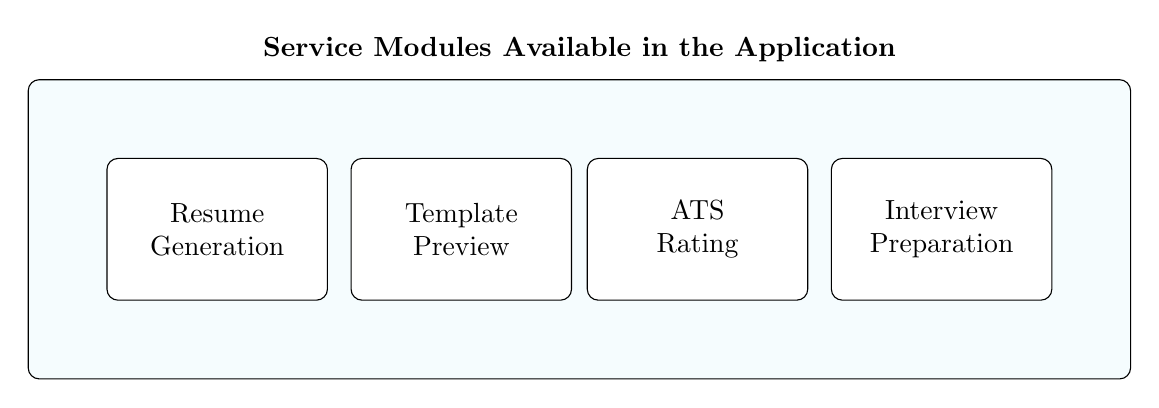
\begin{tikzpicture}[
  shell/.style={draw, rounded corners, minimum width=14cm, minimum height=3.8cm, fill=cyan!4},
  card/.style={draw, rounded corners, minimum width=2.8cm, minimum height=1.8cm, fill=white, align=center}
]
\node[shell] (s) {};
\node[above=0.1cm of s] {\textbf{Service Modules Available in the Application}};
\node[card, xshift=-4.6cm] at (s.center) {Resume\\Generation};
\node[card, xshift=-1.5cm] at (s.center) {Template\\Preview};
\node[card, xshift=1.5cm] at (s.center) {ATS\\Rating};
\node[card, xshift=4.6cm] at (s.center) {Interview\\Preparation};
\end{tikzpicture}
\caption{Overview of the main project modules visible to the user}
\end{figure}

\begin{figure}[H]
\centering
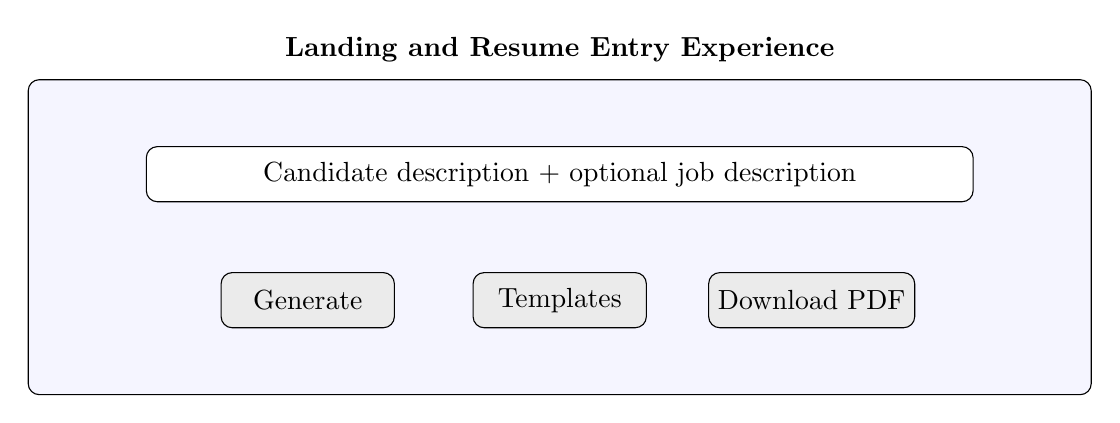
\begin{tikzpicture}[
  screen/.style={draw, rounded corners, minimum width=13.5cm, minimum height=4.0cm, fill=blue!4},
  bar/.style={draw, rounded corners, minimum width=10.5cm, minimum height=0.7cm, fill=white},
  btn/.style={draw, rounded corners, minimum width=2.2cm, minimum height=0.7cm, fill=black!8}
]
\node[screen] (s) {};
\node[above=0.1cm of s] {\textbf{Landing and Resume Entry Experience}};
\node[bar, yshift=0.8cm] at (s.center) {Candidate description + optional job description};
\node[btn, xshift=-3.2cm, yshift=-0.8cm] at (s.center) {Generate};
\node[btn, yshift=-0.8cm] at (s.center) {Templates};
\node[btn, xshift=3.2cm, yshift=-0.8cm] at (s.center) {Download PDF};
\end{tikzpicture}
\caption{Conceptual view of the resume generation workspace}
\end{figure}

\begin{figure}[H]
\centering
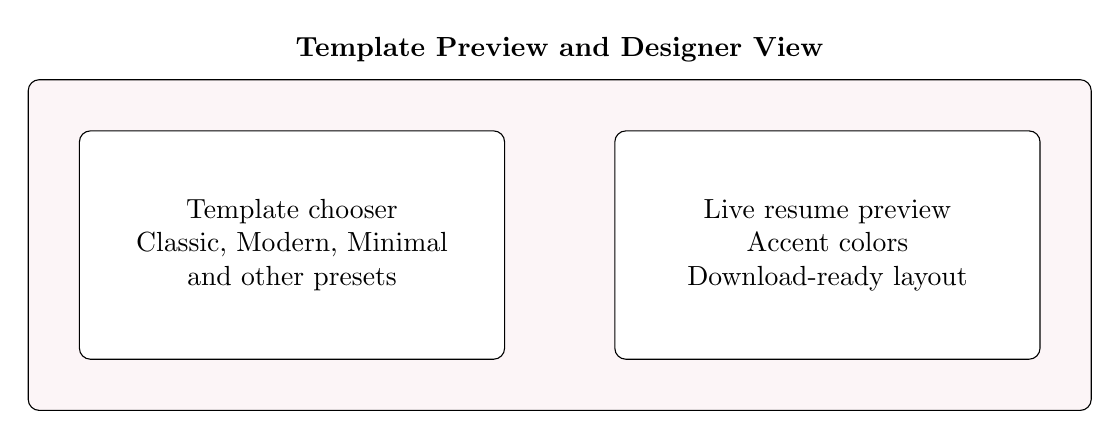
\begin{tikzpicture}[
  screen/.style={draw, rounded corners, minimum width=13.5cm, minimum height=4.2cm, fill=purple!4},
  leftbox/.style={draw, rounded corners, minimum width=5.4cm, minimum height=2.9cm, fill=white, align=center},
  rightbox/.style={draw, rounded corners, minimum width=5.4cm, minimum height=2.9cm, fill=white, align=center}
]
\node[screen] (s) {};
\node[above=0.1cm of s] {\textbf{Template Preview and Designer View}};
\node[leftbox, xshift=-3.4cm] at (s.center) {Template chooser\\Classic, Modern, Minimal\\and other presets};
\node[rightbox, xshift=3.4cm] at (s.center) {Live resume preview\\Accent colors\\Download-ready layout};
\end{tikzpicture}
\caption{Conceptual template selection and designer preview screen}
\end{figure}

\begin{figure}[H]
\centering
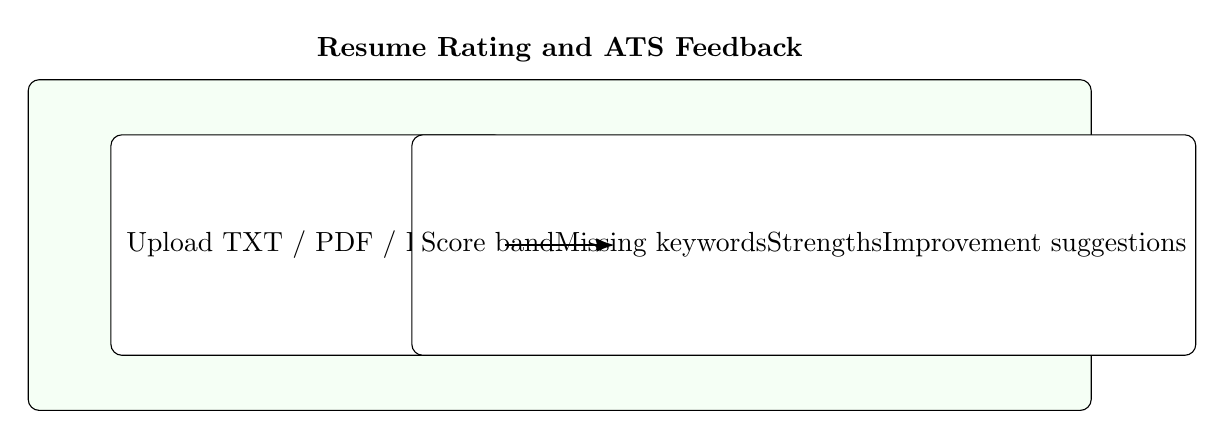
\begin{tikzpicture}[
  screen/.style={draw, rounded corners, minimum width=13.5cm, minimum height=4.2cm, fill=green!4},
  leftbox/.style={draw, rounded corners, minimum width=5.0cm, minimum height=2.8cm, fill=white},
  rightbox/.style={draw, rounded corners, minimum width=6.3cm, minimum height=2.8cm, fill=white}
]
\node[screen] (s) {};
\node[above=0.1cm of s] {\textbf{Resume Rating and ATS Feedback}};
\node[leftbox, xshift=-3.2cm] at (s.center) {Upload TXT / PDF / DOCX};
\node[rightbox, xshift=3.1cm] at (s.center) {Score band\\Missing keywords\\Strengths\\Improvement suggestions};
\draw[-Latex, thick] ([xshift=-0.7cm]s.center) -- ([xshift=0.7cm]s.center);
\end{tikzpicture}
\caption{Conceptual output of the ATS-style resume review module}
\end{figure}

\begin{figure}[H]
\centering
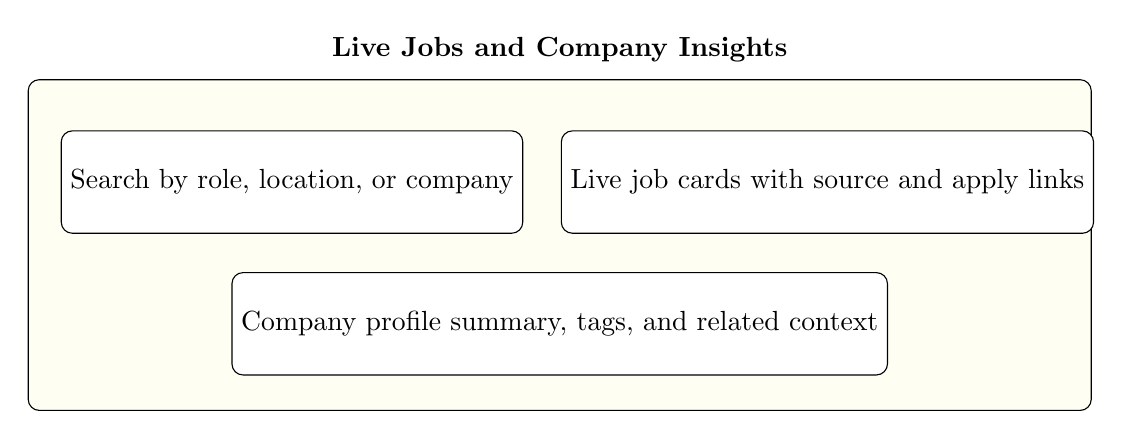
\begin{tikzpicture}[
  screen/.style={draw, rounded corners, minimum width=13.5cm, minimum height=4.2cm, fill=yellow!5},
  box/.style={draw, rounded corners, minimum width=5.2cm, minimum height=1.3cm, fill=white, align=center}
]
\node[screen] (s) {};
\node[above=0.1cm of s] {\textbf{Live Jobs and Company Insights}};
\node[box, xshift=-3.4cm, yshift=0.8cm] at (s.center) {Search by role, location, or company};
\node[box, xshift=3.4cm, yshift=0.8cm] at (s.center) {Live job cards with source and apply links};
\node[box, yshift=-1.0cm] at (s.center) {Company profile summary, tags, and related context};
\end{tikzpicture}
\caption{Conceptual live jobs board and company insight interface}
\end{figure}

\begin{figure}[H]
\centering
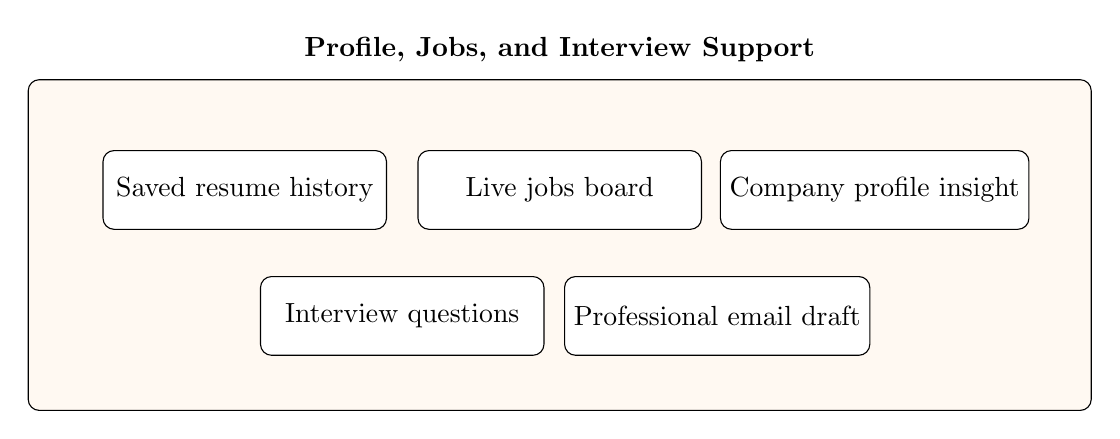
\begin{tikzpicture}[
  screen/.style={draw, rounded corners, minimum width=13.5cm, minimum height=4.2cm, fill=orange!5},
  box/.style={draw, rounded corners, minimum width=3.6cm, minimum height=1.0cm, fill=white}
]
\node[screen] (s) {};
\node[above=0.1cm of s] {\textbf{Profile, Jobs, and Interview Support}};
\node[box, xshift=-4.0cm, yshift=0.7cm] at (s.center) {Saved resume history};
\node[box, xshift=0cm, yshift=0.7cm] at (s.center) {Live jobs board};
\node[box, xshift=4.0cm, yshift=0.7cm] at (s.center) {Company profile insight};
\node[box, xshift=-2.0cm, yshift=-0.9cm] at (s.center) {Interview questions};
\node[box, xshift=2.0cm, yshift=-0.9cm] at (s.center) {Professional email draft};
\end{tikzpicture}
\caption{Conceptual output of supporting career-preparation modules}
\end{figure}

\subsection{Observations}
\noindent The completed application demonstrates that AI assistance becomes more useful when it is combined with structure, persistence, and recruiter-oriented workflows. Instead of acting as a one-time text generator, the system supports an iterative process where the candidate can generate, review, tailor, save, and reuse resume content. This makes the project more practical for real job preparation than a standalone formatting or chatbot-only tool.

\subsection{Feature Outcome Summary}
\begin{table}[H]
\centering
\caption{Outcome summary across major features}
\begin{tabular}{|p{3.6cm}|p{7.0cm}|}
\hline
\textbf{Feature} & \textbf{Practical Outcome} \\
\hline
Resume generation & Converts rough self-description into structured resume sections quickly \\
\hline
Resume tailoring & Improves relevance of content for target job descriptions \\
\hline
ATS-style review & Highlights strengths, missing content, and keyword opportunities \\
\hline
Template preview and export & Produces recruiter-ready PDF output in multiple layouts \\
\hline
Profile storage & Makes it easy to preserve and revisit role-specific resume variants \\
\hline
Interview preparation & Extends the value of the same resume data into prep questions \\
\hline
Live jobs support & Helps users continue directly from resume building into role discovery \\
\hline
\end{tabular}
\end{table}

\subsection{Discussion of Results}
\noindent The results suggest that the most valuable aspect of the project is not any single feature in isolation, but the continuity between features. A candidate can start with incomplete thoughts, convert them into a structured resume, refine the output, compare it against a role, export it, save the version, and continue to job search and interview preparation without switching to a separate system. This continuity reduces repeated data entry and keeps the candidate profile consistent across tasks.

\noindent Another important outcome is the usefulness of structured AI output. Instead of returning a plain paragraph response, the project transforms AI-generated content into fields that map directly to resume sections. This allows the frontend to support edits, template rendering, and export more reliably. In practical terms, the project behaves more like a guided productivity tool than a simple chatbot interface.

\subsection{Limitations of Current Results}
\noindent The observed results are strong for academic and placement-oriented use cases, but they also reflect the current limitations of the implementation. Resume quality still depends on the user’s input quality, local AI execution time may vary with system resources, and live job search depends on upstream providers. These limitations do not invalidate the usefulness of the system, but they define the boundary between the current academic version and a future production-grade deployment.

\newpage
\resetbodyalignment
\section{Conclusion}
\noindent AI Resume Builder successfully brings together resume creation, AI-assisted content generation, ATS-style analysis, template-based export, interview preparation, and job discovery into one integrated system. The project demonstrates how a React frontend and Spring Boot backend can be combined with Spring AI and Ollama to solve a real student and job-seeker problem in a practical way. By structuring model output into reusable resume sections and supporting saved profile history, the application reduces repetitive work and improves the usability of AI in a career-support context.

\noindent The project also shows the value of modular architecture. Authentication, storage, upload analysis, live jobs, and interview preparation are implemented as distinct but connected modules, which makes the application easier to maintain and extend. In future work, the system can be enhanced with stronger recruiter analytics, cover letter generation, richer template theming, collaborative review workflows, and cloud-hosted AI models for faster production-scale performance.

\newpage

\bibliographystyle{IEEEtran}
\bibliography{references}
\newpage

\resetbodyalignment
\section*{Internship Report}
\noindent This project was carried out as a major academic project and provided internship-like exposure to real-world software engineering practices. During the development of AI Resume Builder, the work involved requirement analysis, UI planning, REST API design, AI integration, file-processing support, profile persistence, and report documentation. Even though the project was executed within the academic environment, it closely reflected the responsibilities expected during a full-stack development internship.

\noindent The practical learning outcomes from this work are listed below:
\begin{itemize}
\item Understanding the end-to-end development flow of a modern web application.
\item Building frontend screens with React, routing, forms, and interactive state handling.
\item Designing backend APIs in Spring Boot for authentication, generation, upload analysis, and profile storage.
\item Integrating AI services through Spring AI and Ollama for structured resume generation and interview support.
\item Working with document-processing libraries for PDF and DOCX-based resume analysis.
\item Learning the importance of error handling, modular code organization, and user-focused testing.
\end{itemize}

\noindent Hence, this project served as a strong practical learning experience comparable to an industry-oriented internship in AI-assisted full-stack application development.

\addcontentsline{toc}{section}{Internship Report}
\newpage
\resetbodyalignment
\section*{Publications}
\noindent At the time of submission of this report, no external journal or conference paper has been formally published for the AI Resume Builder project. However, the project has sufficient technical depth and practical relevance to be extended into a future paper in areas such as AI-assisted resume generation, ATS-style resume evaluation, and integrated career-preparation platforms.

\noindent The project is publication-ready in the following directions:
\begin{itemize}
\item AI-assisted generation of structured resumes from free-form candidate descriptions.
\item Comparative study of role-based resume tailoring and keyword matching workflows.
\item Design of an integrated platform combining resume creation, rating, jobs search, and interview preparation.
\item Practical use of Spring AI and local LLM serving for academic and placement-oriented applications.
\end{itemize}

\noindent If a publication is completed later, this section can be updated with the paper title, journal or conference name, authors, acceptance status, and certificate details.

\addcontentsline{toc}{section}{Publication}
\newpage
\resetbodyalignment
\section*{Plagiarism Report}
\noindent This project report titled \textbf{AI Resume Builder} has been checked using a plagiarism-detection tool before final submission. The purpose of this verification is to ensure that the report content is original, properly paraphrased where required, and supported by appropriate citations for referenced technical material, frameworks, and documentation.

\subsection*{Plagiarism Check Summary}
\begin{table}[H]
\centering
\caption{Plagiarism report summary}
\begin{tabular}{|p{4.5cm}|p{7.0cm}|}
\hline
\textbf{Parameter} & \textbf{Details} \\
\hline
Project Title & AI Resume Builder \\
\hline
Student Name & [Student Name] \\
\hline
Exam Seat Number & [Seat Number] \\
\hline
Department & Master of Computer Applications \\
\hline
Plagiarism Checking Tool & [Tool Name] \\
\hline
Date of Check & [DD / MM / YYYY] \\
\hline
Overall Similarity Index & [\% Similarity] \\
\hline
Permissible Limit & [College / University Limit] \\
\hline
Final Status & [Acceptable / Needs Revision] \\
\hline
\end{tabular}
\end{table}

\subsection*{Interpretation}
\noindent The similarity result should be interpreted together with citation quality and the nature of matched text. Technical documents often contain unavoidable similarity in framework names, API terminology, standard definitions, and bibliography entries. Such matches do not necessarily indicate plagiarism when they are properly referenced and used in context. The final report should therefore be reviewed not only for numerical similarity percentage, but also for originality of explanation, project-specific analysis, and correct attribution.

\subsection*{Declaration on Originality}
\noindent The developed system, analysis, design descriptions, implementation details, diagrams, and testing discussion in this report are prepared specifically for the \textbf{AI Resume Builder} project. Wherever external ideas, tools, or documentation have been referred to, those sources are acknowledged in the references section of the report. Any final plagiarism certificate or generated similarity screenshot may be attached below or inserted on the next page at the time of official submission.

\subsection*{Attachment Placeholder}
\noindent Attach the official plagiarism report issued by the checking tool or institution here. If available, insert:
\begin{itemize}
\item similarity percentage screenshot,
\item report ID or scan reference number,
\item date and time of report generation,
\item approval or signature block if required by the department.
\end{itemize}

\addcontentsline{toc}{section}{Plagiarism Report}
\end{document}
